% CMPT 415 Midterm Report
% Compile: tectonic midterm_report.tex  (or pdflatex, run twice for references)
\documentclass[11pt,a4paper]{article}

\usepackage[utf8]{inputenc}
\usepackage[T1]{fontenc}
\usepackage{lmodern}
\usepackage[margin=1in]{geometry}
\usepackage{graphicx}
\usepackage{booktabs}
\usepackage{array}
\usepackage{float}
\usepackage{hyperref}
\usepackage{amsmath}
\usepackage{enumitem}
\usepackage{caption}
\usepackage{subcaption}
\usepackage{xcolor}
\usepackage{tabularx}
\usepackage{multirow}

\hypersetup{
    colorlinks=true,
    linkcolor=blue!70!black,
    citecolor=blue!70!black,
    urlcolor=blue!70!black,
}

\graphicspath{{../artifacts/visualizations/}}

\title{%
  \textbf{CMPT 415 Midterm Report}\\[6pt]
  \Large AI Fairness Dashboard:\\[2pt]
  \large Bias Detection, Qualitative Analysis, and LLM Benchmarking\\
  in Lending Domains
}
\author{
  Siddhant Jain \and Ayaan Lalani
}
\date{\today}

\begin{document}
\maketitle

% ===================================================================
\begin{abstract}
Algorithmic decision-making in lending carries significant fairness risks:
models trained on historical data can perpetuate and amplify biases along
demographic lines. A major goal of this project is to define a
\textbf{reference audit specification}: the set of analysis metrics and
response elements (root causes, severity, concrete recommendations) that
an audit must provide to support remediation. We implement an end-to-end
fairness pipeline applied to two lending datasets (UCI German Credit,
HMDA Georgia), compute five AIF360-based metrics, perform deterministic
qualitative root-cause analysis, and benchmark against an independent
Gemini LLM auditor. Results show moderate bias across most protected
attributes, with pipeline and LLM largely agreeing on severity while
diverging on small subgroups. We plan to benchmark against additional LLMs
to position our approach in the broader landscape.
\end{abstract}

% ===================================================================
\section{Introduction}

Automated lending decisions (credit scoring, mortgage approvals, loan
pricing) increasingly rely on machine learning models. While these models
improve efficiency, they risk encoding historical biases present in
training data, leading to disparate outcomes for protected groups defined
by sex, age, race, or national origin.

Regulatory frameworks such as the U.S.\ Equal Credit Opportunity Act (ECOA)
and the EU AI Act mandate that lending models be audited for discriminatory
impact. However, detecting bias requires more than a single metric: it
demands multi-dimensional quantitative measurement, qualitative root-cause
analysis, and independent validation.

\paragraph{Interim problem statement.}
We focus on evaluating biases in datasets and, over time, in the data used
by AI models, in order to provide recommendations on how to fix those
biases so that future systems do not exhibit them. Lending is our current
application domain; the framing aims to be applicable to any domain where
biased data or models lead to unfair outcomes (e.g., lending, hiring)
eventually.

\paragraph{Major goals.}
Two goals drive this work. First, we aim to define a \textbf{reference
audit specification}: the set of analysis metrics and response elements
(root causes, severity, concrete mitigation recommendations) that a
fairness audit must provide so that remediations can be carried out. This
specification answers: what to measure, how to interpret it, and what to
recommend. Second, we aim to \textbf{benchmark against multiple LLMs} (we
start with Gemini and plan to add others) so that we can see where our
deterministic pipeline stands in the general scheme of things and when to
prefer or combine rule-based vs.\ LLM-based analysis.

This project makes three contributions:
\begin{enumerate}[nosep]
  \item A \textbf{reproducible fairness pipeline} that preprocesses data,
        trains classifiers, computes five AIF360-based metrics, and generates
        structured reports aligned with the reference audit specification.
  \item A \textbf{deterministic qualitative analysis engine} that diagnoses
        data imbalance, detects proxy features, maps root causes, and
        recommends specific mitigations.
  \item An \textbf{LLM benchmark} (Gemini initially; more LLMs planned) that
        independently audits the same prediction data using fairlearn
        definitions, enabling side-by-side comparison and positioning of our
        approach relative to LLM-based auditors.
\end{enumerate}

% ===================================================================
\section{Background and Related Work}

\subsection{Fairness Metrics}

We adopt five widely-used group fairness metrics. Let $\hat{Y}$ denote
predictions, $Y$ ground truth, and $A$ the protected attribute with
privileged group $a_p$ and unprivileged group $a_u$.

\begin{itemize}[nosep]
  \item \textbf{Disparate Impact (DI)}: ratio of selection rates.
        $\text{DI} = P(\hat{Y}{=}1 \mid A{=}a_u)\;/\;P(\hat{Y}{=}1 \mid A{=}a_p)$.
        Values below 0.8 indicate adverse impact (four-fifths rule).
  \item \textbf{Demographic Parity Difference (DPD)}: difference of selection
        rates, $P(\hat{Y}{=}1 \mid A{=}a_u) - P(\hat{Y}{=}1 \mid A{=}a_p)$.
  \item \textbf{Equal Opportunity Difference (EOD)}: difference of true
        positive rates,
        $\text{TPR}(a_u) - \text{TPR}(a_p)$.
  \item \textbf{Average Odds Difference (AOD)}:
        $\frac{1}{2}[(\text{FPR}(a_u){-}\text{FPR}(a_p)) +
        (\text{TPR}(a_u){-}\text{TPR}(a_p))]$.
  \item \textbf{Theil Index}: an entropy-based inequality measure over
        predicted benefits.
\end{itemize}

\subsection{Fairness Toolkits}

\textbf{AIF360}~\cite{aif360} (IBM) provides dataset wrappers, metric
classes, and pre-/in-/post-processing mitigation algorithms.
\textbf{Fairlearn}~\cite{fairlearn} (Microsoft) offers constraint-based
reduction algorithms (\texttt{ExponentiatedGradient}, \texttt{GridSearch})
and the \texttt{ThresholdOptimizer} post-processor. Our deterministic
pipeline uses AIF360 metric definitions, while the LLM benchmark is
constrained to fairlearn.

\subsection{LLMs as Fairness Auditors}

Recent work has explored using large language models to interpret model
behavior and generate natural-language explanations of bias. We benchmark
this approach by sending raw prediction data to Google's Gemini 2.5 Flash
model and comparing its independently computed metrics and qualitative
conclusions against our deterministic pipeline.

% ===================================================================
\section{Datasets}

\subsection{German Credit Dataset}

The UCI Statlog German Credit dataset contains 1{,}000 consumer credit
records. We merge the original Statlog encoding with a Kaggle-hosted
version to obtain human-readable feature names. Protected attributes are
derived as follows:
\begin{itemize}[nosep]
  \item \textbf{Sex}: extracted from personal status codes (Attribute~9).
  \item \textbf{AgeGroup}: binarized at 40 ($<$40 $\rightarrow$ \texttt{under\_40}, $\geq$40 $\rightarrow$ \texttt{40\_plus}).
  \item \textbf{Foreign Worker}: extracted from Attribute~20 (A201/A202 encoding).
\end{itemize}
The target variable is credit reliability (1~=~good, 0~=~bad). An 80/20
train-test split yields 200 test records for fairness evaluation.

\subsection{HMDA Mortgage Lending (Georgia)}

The Home Mortgage Disclosure Act requires U.S.\ lenders to report
application-level data. We download 2022 Georgia records from the
CFPB Data Browser API, filtering to originated and denied applications.
After cleaning and sampling, the dataset contains 6{,}525 records.
Protected attributes:
\begin{itemize}[nosep]
  \item \textbf{Race}: White, Black, Asian, American Indian, Pacific Islander, Multiracial.
  \item \textbf{Sex}: Male, Female.
  \item \textbf{Age Group}: young ($<$35), mid (35--54), senior ($\geq$55).
\end{itemize}
The target is loan approval (1~=~originated, 0~=~denied). A 2{,}196-record
test set is used for evaluation.

\begin{table}[H]
\centering
\caption{Dataset summary.}
\label{tab:datasets}
\resizebox{\textwidth}{!}{%
\begin{tabular}{lrrrrlp{2.2cm}r}
\toprule
\textbf{Dataset} & \textbf{Records} & \textbf{Test} & \textbf{Feat.} & \textbf{Prot.\ Attrs} & \textbf{Target} & \textbf{\% Fav.} \\
\midrule
German Credit    & 1{,}000 & 200   & 10 & 3 (Sex, Age, Foreign) & Credit reliability & 70\% \\
HMDA (Georgia)   & 6{,}525 & 2{,}196 & 8  & 3 (Race, Sex, Age)    & Loan approval      & 72\% \\
\bottomrule
\end{tabular}%
}
\end{table}

% ===================================================================
\section{Methodology}

\subsection{Pipeline Architecture}

All analysis is orchestrated by a central pipeline (\texttt{run\_pipeline.py})
that executes six sequential steps per dataset:

\begin{center}
\texttt{clean} $\rightarrow$ \texttt{train} $\rightarrow$
\texttt{fairness} $\rightarrow$ \texttt{qualitative} $\rightarrow$
\texttt{llm\_benchmark} $\rightarrow$ \texttt{visualize}
\end{center}

A consolidation step then merges per-dataset results into cross-dataset
reports and comparison visualizations. The pipeline supports selective
execution (e.g., rerunning only the LLM benchmark step).

\subsection{Reference Audit Specification}

To support remediation, we define a \textbf{reference audit specification}:
the minimum set of metrics and response elements that an analysis must
provide. \textbf{Metrics:} (1) Disparate Impact, (2) Demographic Parity
Difference, (3) Equal Opportunity Difference, (4) Average Odds Difference,
(5) Theil Index; each per protected attribute with privileged/unprivileged
groups stated. \textbf{Response elements:} (1) per-group breakdown
(selection rate, TPR, FPR, base rate); (2) severity classification
(Critical / High / Moderate / Low) with a stated threshold (e.g., DI$<$0.8);
(3) diagnosed root causes (e.g., data imbalance, proxy features, historical
label bias); (4) concrete mitigation recommendations (algorithm or
post-processing step). Our pipeline and our comparison with LLMs are
evaluated against this specification; future work will benchmark
additional LLMs on the same specification.

\subsection{Model Training}

For each dataset, we train two classifiers (Logistic Regression and
Random Forest) using scikit-learn. Continuous features are standardized
(\texttt{StandardScaler}), categorical features are label-encoded, and
missing values are imputed with the mode. We use an 80/20 stratified
train-test split. Predictions on the test set are exported with original
protected attribute labels preserved for downstream fairness analysis.

\subsection{Fairness Metric Computation}

For each protected attribute, we define the privileged group based on
domain knowledge (Table~\ref{tab:priv}). Five metrics are computed:
DI, DPD, EOD, AOD, and Theil Index. A bias flag is raised when
DI~$<$~0.8. Results are exported to CSV and Markdown reports.

\begin{table}[H]
\centering
\caption{Privileged group definitions.}
\label{tab:priv}
\begin{tabular}{llll}
\toprule
\textbf{Dataset} & \textbf{Attribute} & \textbf{Privileged} & \textbf{Rationale} \\
\midrule
German Credit & Sex              & Male     & Historically advantaged in credit \\
              & AgeGroup         & 40+      & Longer credit history \\
              & Foreign Worker   & Non-foreign (0) & Domestic applicants favored \\
\midrule
HMDA          & Race             & White    & Majority, historically favored \\
              & Sex              & Male     & Historically advantaged \\
              & Age Group        & Mid (35--54) & Peak earning years \\
\bottomrule
\end{tabular}
\end{table}

\subsection{Qualitative Analysis Engine}

Our deterministic qualitative module (\texttt{qualitative\_analysis.py})
performs four analyses per protected attribute:

\begin{enumerate}[nosep]
  \item \textbf{Per-group breakdown}: selection rates, TPR, FPR, and base
        rates for every subgroup.
  \item \textbf{Data imbalance diagnosis}: flags group size ratios
        $>$3$\times$, groups with $<$30 records, and base-rate disparities
        $>$15\%.
  \item \textbf{Proxy feature detection}: computes point-biserial
        correlation (binary attributes) or eta-squared (multi-class) between
        each numeric feature and the protected attribute, flagging
        correlations $\geq$0.15.
  \item \textbf{Root-cause mapping}: a rule engine maps metric patterns
        (e.g., $|\text{EOD}| > 0.05$) and detected proxies to specific root
        causes and AIF360 mitigation algorithms.
\end{enumerate}

Each attribute receives a severity classification: \textsc{Critical}
(DI~$<$~0.72), \textsc{High} (0.72--0.80), \textsc{Moderate} (0.80--0.95),
or \textsc{Low} ($\geq$0.95).

\subsection{LLM Benchmark}

The LLM benchmark sends \emph{only} the raw predictions CSV (ground truth,
predicted labels, and protected attribute columns) to Google's Gemini 2.5
Flash model. The prompt instructs Gemini to:
\begin{itemize}[nosep]
  \item Compute DI, DPD, EOD, AOD, and Theil Index using \textbf{fairlearn}
        metric definitions.
  \item Produce qualitative analysis: what is wrong, why, and how to fix it
        using fairlearn mitigation algorithms.
  \item Return structured JSON for programmatic comparison.
\end{itemize}
Critically, the LLM receives \textbf{zero access} to our pre-computed
metrics, qualitative report, or AIF360-based calculations. The comparison
is then generated by our pipeline, which loads both sets of results
independently.

% ===================================================================
\section{Results}

\subsection{German Credit: Fairness Metrics}

\begin{table}[H]
\centering
\caption{German Credit fairness metrics (our pipeline).}
\label{tab:gc-metrics}
\begin{tabular}{lccccc}
\toprule
\textbf{Attribute} & \textbf{DI} & \textbf{DPD} & \textbf{EOD} & \textbf{AOD} & \textbf{Theil} \\
\midrule
Sex (priv: male)              & 0.8595 & $-$0.1152 & $-$0.0512 & $-$0.1256 & 0.3084 \\
AgeGroup (priv: 40+)          & 0.8212 & $-$0.1586 & $-$0.0513 & $-$0.1649 & 0.3084 \\
Foreign Worker (priv: non-fw)  & 0.9402 & $-$0.0498 & $-$0.0889 & $+$0.2013 & 0.3084 \\
\bottomrule
\end{tabular}
\end{table}

All three attributes fall in the \textsc{Moderate} severity range
(DI between 0.80 and 0.95). Sex and AgeGroup show consistent disadvantage
for the unprivileged group across all metrics. Foreign Worker metrics are
unreliable due to extreme group imbalance (194 vs.\ 6 records).

\begin{figure}[H]
\centering
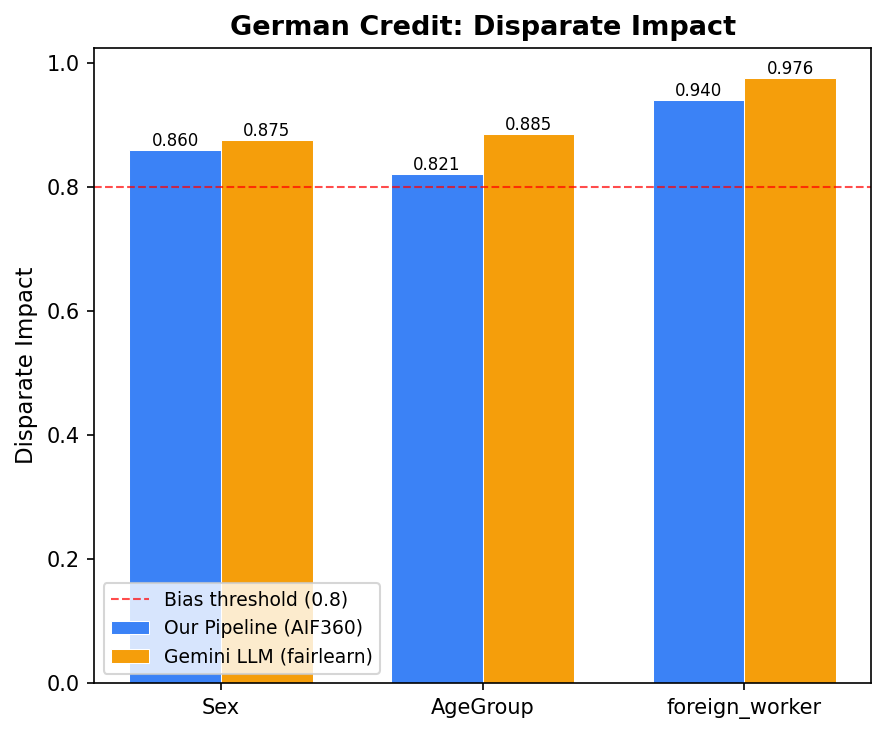
\includegraphics[width=0.85\textwidth]{german_credit_disparate_impact.png}
\caption{German Credit: Disparate Impact by protected attribute
         (pipeline vs.\ LLM).}
\label{fig:gc-di}
\end{figure}

\subsection{HMDA: Fairness Metrics}

\begin{table}[H]
\centering
\caption{HMDA (Georgia) fairness metrics (our pipeline).}
\label{tab:hmda-metrics}
\begin{tabular}{lccccc}
\toprule
\textbf{Attribute} & \textbf{DI} & \textbf{DPD} & \textbf{EOD} & \textbf{AOD} & \textbf{Theil} \\
\midrule
Race (priv: White)     & 0.8956 & $-$0.0776 & $+$0.0025 & $+$0.0117 & 0.4838 \\
Sex (priv: Male)       & 0.9291 & $-$0.0518 & $-$0.0076 & $-$0.0084 & 0.4838 \\
Age Group (priv: mid)  & 1.0138 & $+$0.0097 & $+$0.0008 & $-$0.0150 & 0.4838 \\
\bottomrule
\end{tabular}
\end{table}

Race exhibits \textsc{Moderate} bias (DI~=~0.8956), sex is borderline
\textsc{Moderate} (DI~=~0.9291), and age group is effectively fair
(DI~=~1.0138). The small EOD and AOD values for HMDA suggest the model's
error rates are relatively balanced across groups, with the primary
disparity being in overall selection rates.

\begin{figure}[H]
\centering
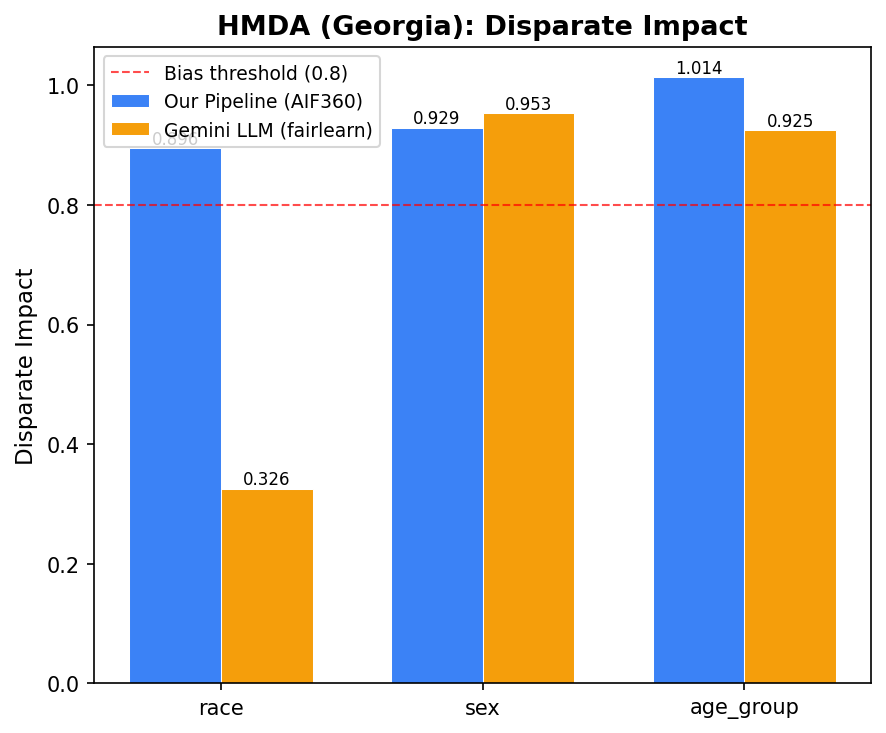
\includegraphics[width=0.85\textwidth]{hmda_disparate_impact.png}
\caption{HMDA: Disparate Impact by protected attribute
         (pipeline vs.\ LLM).}
\label{fig:hmda-di}
\end{figure}

\subsection{Qualitative Findings}

The qualitative engine identified the following root causes:

\paragraph{German Credit.}
\begin{itemize}[nosep]
  \item \textbf{Sex}: Strong proxy feature detected (\texttt{Sex} column,
        $r{=}1.0$); the encoded Sex feature directly leaks into the model.
        Weaker proxies include Housing ($r{=}{-}0.27$) and Age ($r{=}0.22$).
        Root causes: proxy discrimination, unequal opportunity
        (EOD~$=$~$-$0.05), and unequal odds (AOD~$=$~$-$0.13).
  \item \textbf{AgeGroup}: Strong proxy via Age ($r{=}{-}0.84$) and the
        AgeGroup encoding itself. Historical label bias detected: 40+
        borrowers have a 77.5\% favorable base rate vs.\ 65.9\% for under-40.
  \item \textbf{Foreign Worker}: Severe size imbalance (194 vs.\ 6 records,
        32$\times$ ratio). Metrics for the non-foreign group are statistically
        unreliable ($n{=}6$). Root cause: representation bias.
\end{itemize}

\paragraph{HMDA.}
\begin{itemize}[nosep]
  \item \textbf{Race}: Severe size imbalance (White: 1{,}252 vs.\ Pacific
        Islander: 5, a 250$\times$ ratio). Base-rate disparity: Asian
        applicants have 79.8\% favorable outcomes vs.\ Multiracial at 37.5\%
        (gap~$=$~42.3\%). Root causes: historical/label bias and
        representation bias.
  \item \textbf{Sex}: Borderline disparity with no strong root cause
        detected by the rule engine. Recommended: post-processing threshold
        calibration.
  \item \textbf{Age Group}: No significant disparity (DI~$>$~1.0), though
        historical label bias exists in the ground truth.
\end{itemize}

\subsection{LLM Benchmark Comparison}

\subsubsection{Metric Comparison}

\begin{table}[H]
\centering
\caption{Metric comparison: Our Pipeline (AIF360) vs.\ Gemini LLM (fairlearn).}
\label{tab:benchmark}
\small
\begin{tabular}{llrrr}
\toprule
\textbf{Attribute} & \textbf{Metric} & \textbf{Ours} & \textbf{Gemini} & \textbf{$\Delta$} \\
\midrule
\multicolumn{5}{l}{\textit{German Credit}} \\
Sex             & DI  & 0.8595 & 0.8752 & $+$0.016 \\
                & DPD & $-$0.1152 & $-$0.0988 & $+$0.016 \\
                & EOD & $-$0.0512 & $-$0.0658 & $-$0.015 \\
                & AOD & $-$0.1256 & $-$0.0381 & $+$0.088 \\
AgeGroup        & DI  & 0.8212 & 0.8848 & $+$0.064 \\
                & DPD & $-$0.1586 & $-$0.0950 & $+$0.064 \\
                & EOD & $-$0.0513 & $-$0.0811 & $-$0.030 \\
                & AOD & $-$0.1649 & $-$0.0245 & $+$0.140 \\
Foreign Worker  & DI  & 0.9402 & 0.9755 & $+$0.035 \\
\midrule
\multicolumn{5}{l}{\textit{HMDA (Georgia)}} \\
Race            & DI  & 0.8956 & 0.3258 & $-$0.570 \\
                & DPD & $-$0.0776 & $-$0.5173 & $-$0.440 \\
Sex             & DI  & 0.9291 & 0.9532 & $+$0.024 \\
Age Group       & DI  & 1.0138 & 0.9254 & $-$0.088 \\
\bottomrule
\end{tabular}
\end{table}

\subsubsection{Severity Agreement}

\begin{table}[H]
\centering
\caption{Severity classification agreement.}
\label{tab:severity}
\begin{tabular}{llccl}
\toprule
\textbf{Dataset} & \textbf{Attribute} & \textbf{Ours} & \textbf{Gemini} & \textbf{Agree?} \\
\midrule
German Credit & Sex              & Moderate & Moderate  & Yes \\
              & AgeGroup         & Moderate & Moderate  & Yes \\
              & Foreign Worker   & Moderate & Low       & No \\
\midrule
HMDA          & Race             & Moderate & Critical  & No \\
              & Sex              & Moderate & Low       & No \\
              & Age Group        & Low      & Low       & Yes \\
\bottomrule
\end{tabular}
\end{table}

\begin{figure}[H]
\centering
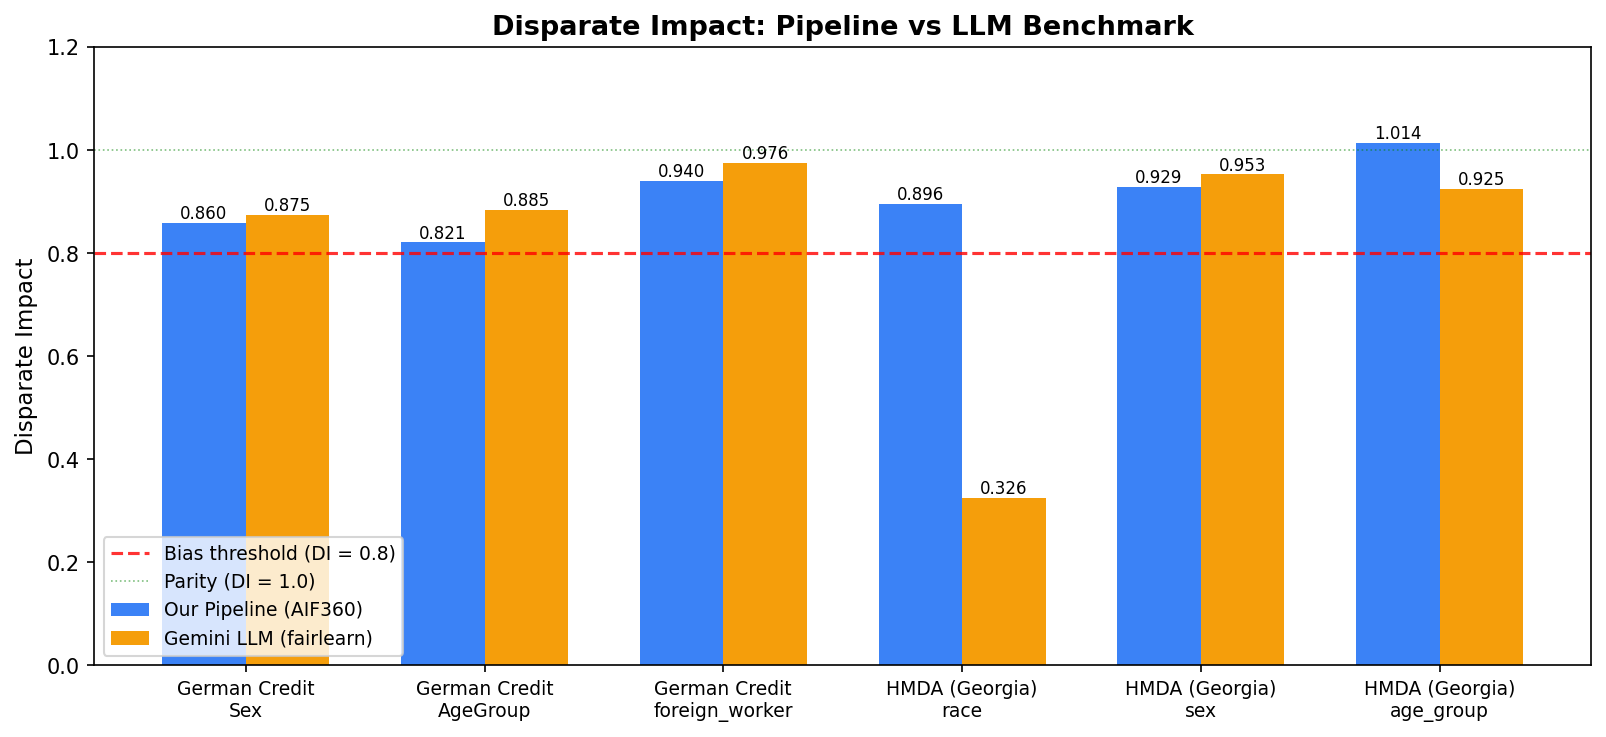
\includegraphics[width=\textwidth]{di_overview.png}
\caption{Disparate Impact overview across all datasets and attributes.}
\label{fig:di-overview}
\end{figure}

\begin{figure}[H]
\centering
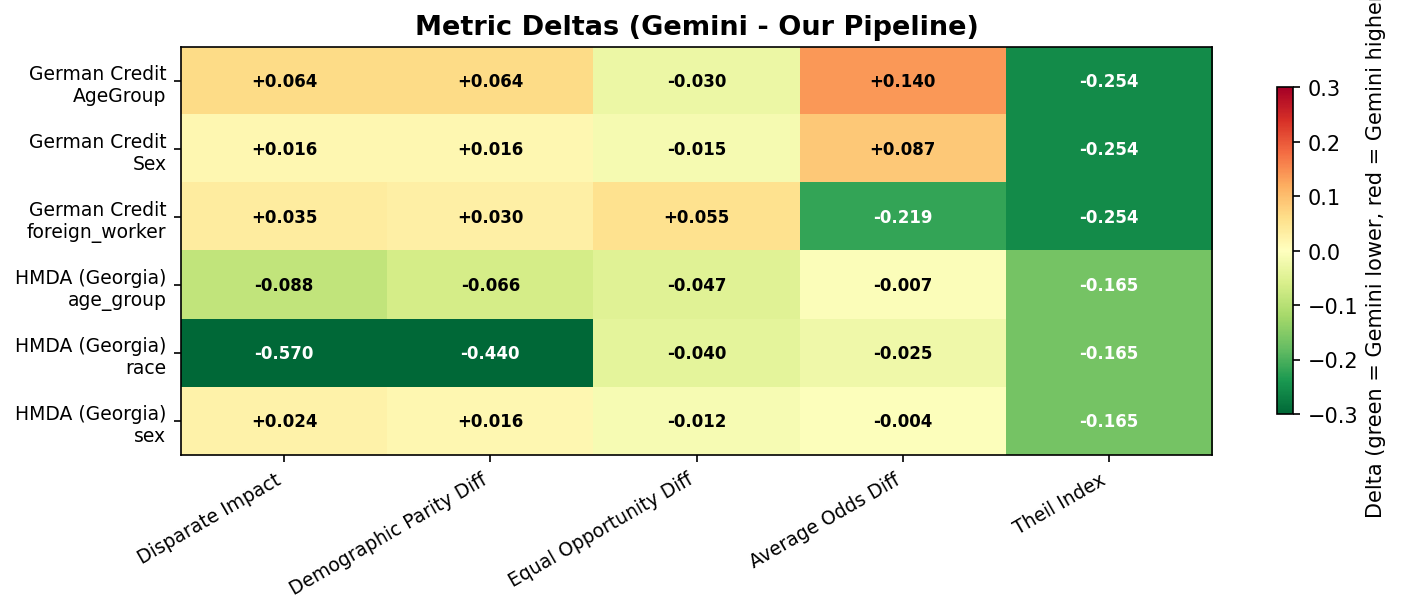
\includegraphics[width=\textwidth]{delta_heatmap.png}
\caption{Metric deltas (Gemini $-$ Our Pipeline). Red indicates Gemini
         computed a higher value; green indicates lower.}
\label{fig:delta-heatmap}
\end{figure}

\begin{figure}[H]
\centering
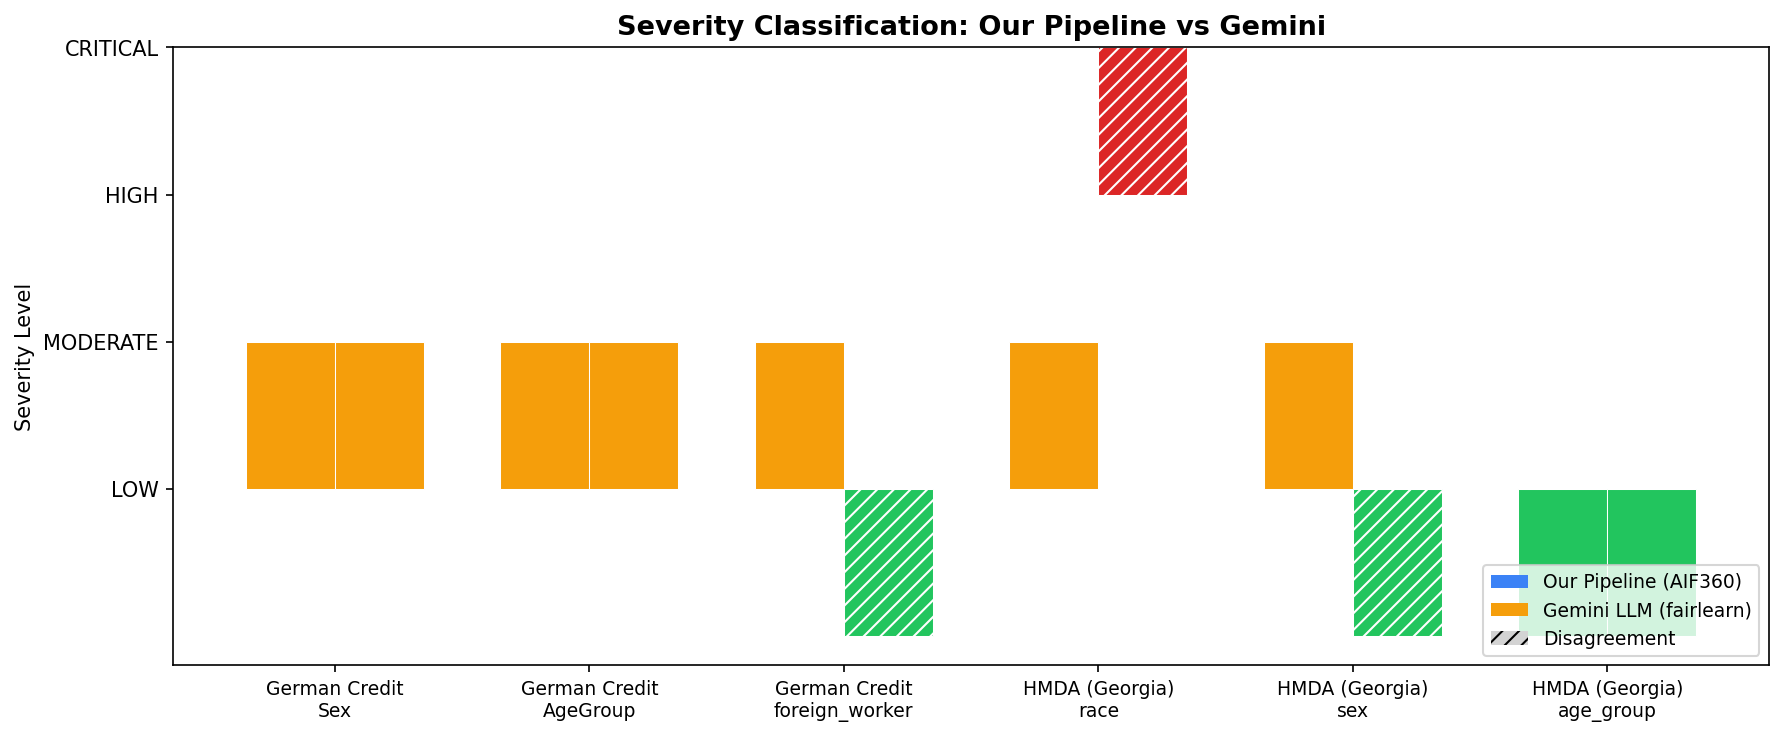
\includegraphics[width=0.9\textwidth]{severity_comparison.png}
\caption{Severity classification comparison. Hatched bars indicate
         disagreement between the two approaches.}
\label{fig:severity}
\end{figure}

\subsection{Cost Analysis}

\begin{table}[H]
\centering
\caption{LLM benchmark cost breakdown (Gemini 2.5 Flash).}
\label{tab:cost}
\resizebox{\textwidth}{!}{%
\begin{tabular}{lrrrr}
\toprule
\textbf{Dataset} & \textbf{Input Tok.} & \textbf{Output Tok.} & \textbf{Latency (s)} & \textbf{Est.\ Cost} \\
\midrule
German Credit & 3{,}539   & 1{,}904 & 75.6  & \$0.0011 \\
HMDA          & 22{,}910  & 1{,}826 & 121.6 & \$0.0030 \\
\midrule
\textbf{Total} & 26{,}449 & 3{,}730 & 197.2 & \textbf{\$0.0041} \\
\bottomrule
\end{tabular}%
}
\end{table}

The total cost for auditing both datasets is under half a cent, making
LLM-based fairness auditing economically viable even for frequent re-runs.

\begin{figure}[H]
\centering
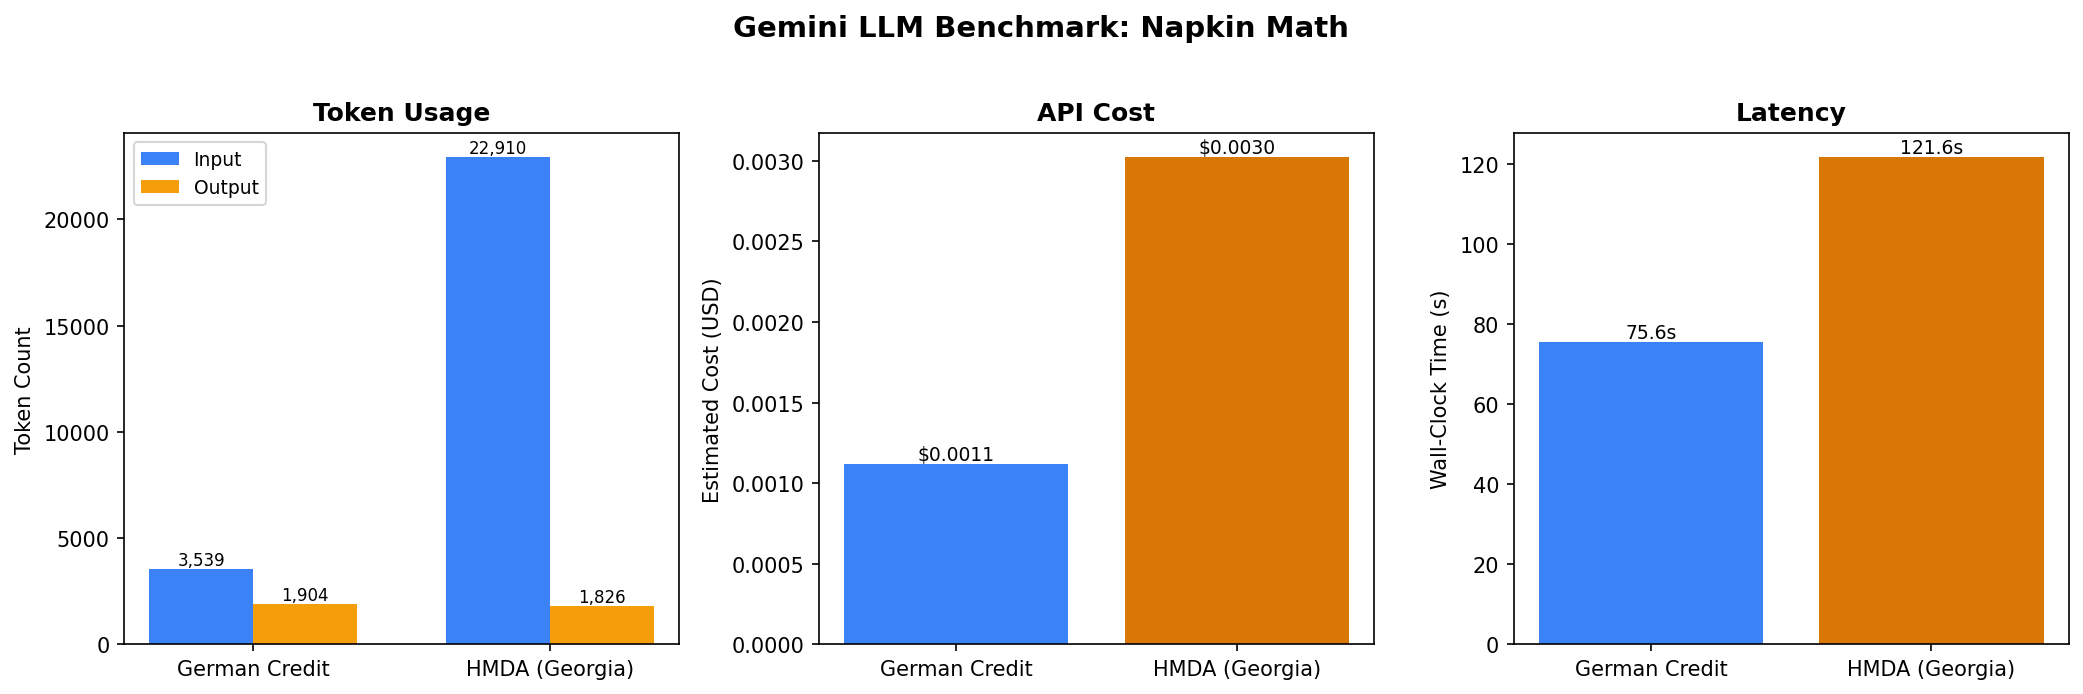
\includegraphics[width=\textwidth]{cost_summary.png}
\caption{Token usage, API cost, and latency per dataset.}
\label{fig:cost}
\end{figure}

% ===================================================================
\section{Discussion}

\subsection{Where Pipeline and LLM Agree}

For the German Credit dataset, both approaches agree on severity for Sex
and AgeGroup (\textsc{Moderate}) and produce directionally consistent
metrics (DI, DPD, EOD all negative for unprivileged groups). This
validates that both AIF360 and fairlearn metric definitions, when applied
to the same data, yield similar conclusions for well-balanced binary
attributes.

\subsection{Where They Diverge}

The most significant divergence occurs on HMDA Race, where our pipeline
reports DI~$=$~0.8956 (\textsc{Moderate}) while Gemini reports
DI~$=$~0.3258 (\textsc{Critical}). The root cause is \textbf{unprivileged
group selection}: our pipeline computes DI using a weighted average across
unprivileged groups (AIF360 convention), while Gemini selected the
single worst-performing group (American Indian, $n{=}10$) as the
unprivileged baseline. With only 10 records, this group's selection rate
(0.40) is statistically noisy, producing an alarming but unreliable DI.

This highlights a key risk of LLM-based auditing: \textbf{the LLM lacks
statistical reasoning about sample sizes}. Our deterministic pipeline's
imbalance diagnosis explicitly flags groups with $<$30 records as
unreliable, while Gemini treats all groups equally regardless of size.

\subsection{Strengths and Limitations}

\paragraph{Deterministic pipeline.}
Strengths: fully reproducible, transparent rule logic, specific AIF360
mitigation recommendations, statistical safeguards (minimum group size,
confidence warnings). Limitations: rigid rule structure cannot capture
novel bias patterns; qualitative explanations are templated.

\paragraph{LLM benchmark.}
Strengths: richer, more natural-language explanations; can identify
context-specific issues (e.g., zip-code-as-proxy for race in mortgage
lending). Limitations: generic mitigation advice (same fairlearn
recommendations repeated per attribute); no statistical reasoning about
sample sizes; non-deterministic (different runs may yield different
metrics); higher latency (75--122s vs.\ $<$1s for our pipeline).

\subsection{Value of Qualitative Analysis}

Raw fairness metrics alone are insufficient for actionable remediation.
A DI of 0.82 does not explain \emph{why} the model is biased or
\emph{what to do about it}. Our qualitative engine bridges this gap:
for AgeGroup, it identifies that (a) the Age feature is a strong proxy
($r{=}{-}0.84$), (b) ground-truth labels embed historical age
discrimination, and (c) specific AIF360 algorithms
(Reweighing, DisparateImpactRemover) can address these root causes.

% ===================================================================
\section{Conclusion and Future Work}

We presented a multi-layered fairness auditing system for lending models
combining quantitative metrics, deterministic qualitative analysis, and
LLM-based independent benchmarking. Key findings:
\begin{itemize}[nosep]
  \item Both German Credit and HMDA exhibit \textsc{Moderate} bias on
        most protected attributes, driven by historical label disparities
        and proxy features.
  \item The deterministic pipeline and Gemini LLM agree on severity for
        4 of 6 attribute-dataset pairs, with disagreements traceable to
        methodological differences in handling multi-group attributes and
        small subgroups.
  \item LLM auditing is economically viable (\$0.004 total) but requires
        guardrails for statistical reasoning that deterministic systems
        provide natively.
\end{itemize}

\paragraph{Future work.}
We plan to: (1) formulate andformalize the reference audit specification so
that other tools and LLMs can be evaluated against it; (2) benchmark
against additional LLMs (e.g., Claude, GPT, open-weight models) on the
same prediction data and prompt structure to see where our pipeline stands
in the general scheme of things; (3) deepen analysis within the finance and
lending domain first via in-depth analysis of the two datasets we have used so far, and then via additional datasets if required (peer-to-peer lending, credit
bureau data), intersectional fairness (e.g., race $\times$ sex), and
end-to-end mitigation (implementing Reweighing, ExponentiatedGradient,
ThresholdOptimizer and measuring accuracy-fairness trade-offs); (4) add
longitudinal bias monitoring to detect fairness drift over time.

% ===================================================================
\begin{thebibliography}{9}

\bibitem{aif360}
R.~K.~E.~Bellamy et~al.,
``AI Fairness 360: An extensible toolkit for detecting and mitigating
algorithmic bias,''
\textit{IBM Journal of Research and Development}, vol.~63, no.~4/5, 2019.
\url{https://github.com/Trusted-AI/AIF360}

\bibitem{fairlearn}
S.~Bird et~al.,
``Fairlearn: A toolkit for assessing and improving fairness in AI,''
Microsoft Research, Tech.\ Rep., 2020.
\url{https://fairlearn.org}

\bibitem{german}
H.~Hofmann,
``Statlog (German Credit Data),''
UCI Machine Learning Repository, 1994.
\url{https://archive.ics.uci.edu/ml/datasets/statlog+(german+credit+data)}

\bibitem{hmda}
Consumer Financial Protection Bureau,
``HMDA Data Browser,''
\url{https://ffiec.cfpb.gov/data-browser/}

\bibitem{gemini}
Google DeepMind,
``Gemini API Documentation,''
\url{https://ai.google.dev/docs}

\end{thebibliography}

\end{document}
